% =====================================================================
%  Chapitre 3 -- partie c : optimisation, extensions, pieges
% =====================================================================

\begin{frame}{Comment on ajuste en pratique : descente de gradient}
\begin{columns}[t]
\begin{column}{0.52\textwidth}
\centering
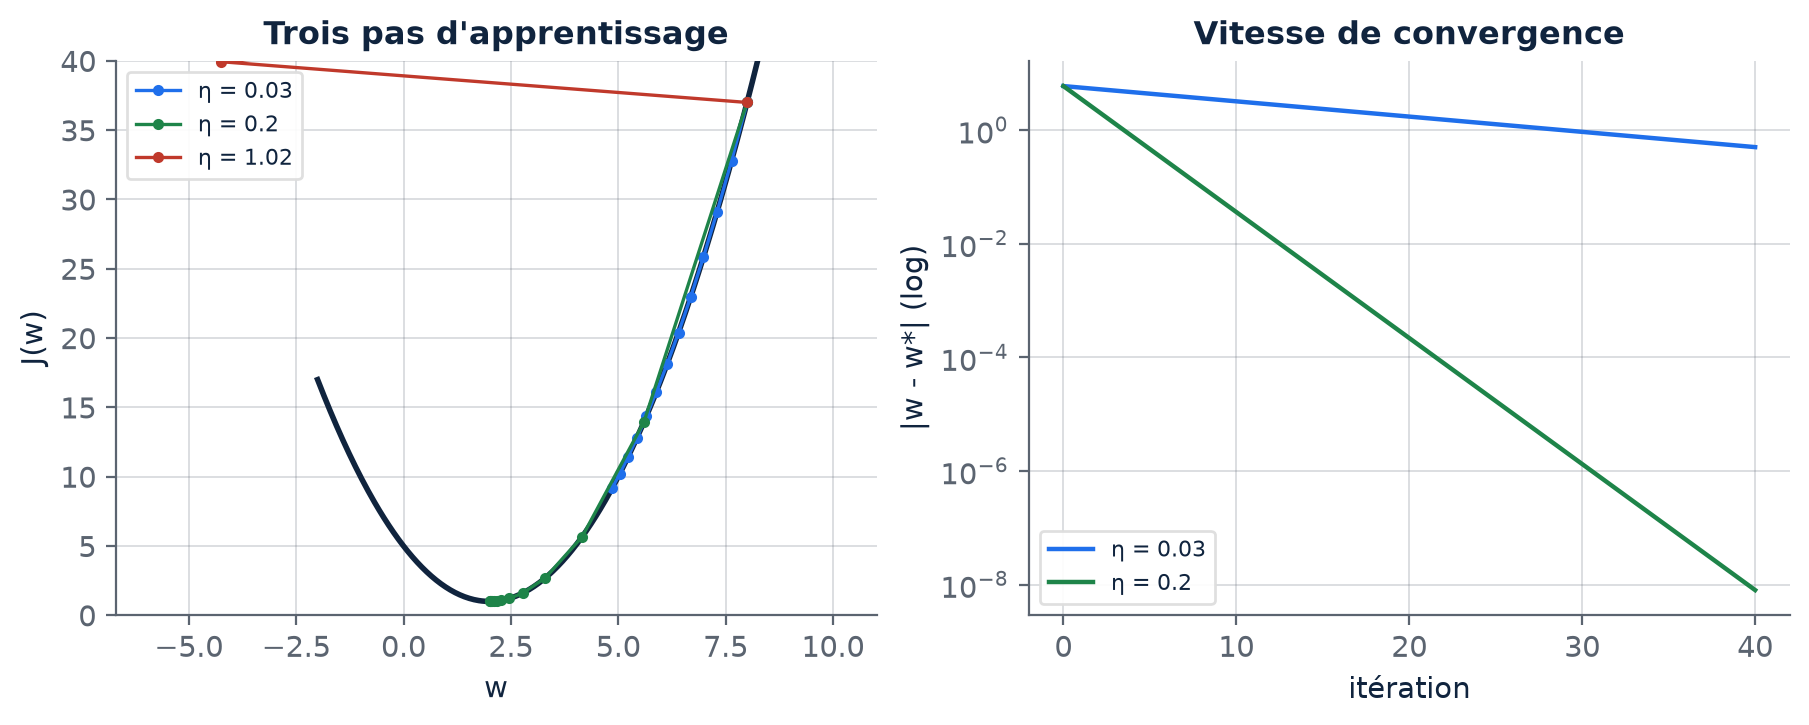
\includegraphics[height=0.29\textheight,keepaspectratio]{k05_descente.png}
\end{column}
\begin{column}{0.44\textwidth}
\[
  \beta^{(t+1)}=\beta^{(t)}-\eta\,\nabla L(\beta^{(t)})
\]
\begin{itemize}
  \item $\eta=0{,}03$ : convergence lente --- écart final $0{,}505$.
  \item $\eta=0{,}2$ : convergence en quelques dizaines d'itérations ---
        écart final $0{,}000$.
  \item $\eta$ trop grand : divergence.
\end{itemize}
\end{column}
\end{columns}
\vspace{1mm}
\begin{kbox}[Pourquoi on l'utilise encore]
La forme fermée coûte $O(p^3)$ et devient impraticable au-delà de quelques
milliers de variables. La descente de gradient passe à l'échelle.
\end{kbox}
\end{frame}

\begin{frame}{Trois variantes de descente}
\begin{center}
\small
\begin{tabular}{@{}p{0.18\textwidth}p{0.30\textwidth}p{0.40\textwidth}@{}}
\toprule
\textbf{Variante} & \textbf{Calcul du gradient sur} & \textbf{Propriété} \\
\midrule
Batch & tous les exemples & stable, coûteux par itération \\
Stochastique (SGD) & un seul exemple & bruité, très rapide, converge bien \\
Mini-batch & 32 à 256 exemples & compromis utilisé partout \\
\bottomrule
\end{tabular}
\end{center}
\vspace{2mm}
\begin{columns}[t]
\begin{column}{0.48\textwidth}
\begin{kbox}[Le bruit de SGD n'est pas un défaut]
Il aide à sortir des points selle et des minima locaux.
\end{kbox}
\end{column}
\begin{column}{0.48\textwidth}
\begin{wbox}[Le piège du pas]
Un pas trop grand fait osciller, puis diverger. On le réduit au fil des
époques (\emph{learning rate decay}).
\end{wbox}
\end{column}
\end{columns}
\end{frame}

\begin{frame}{Aller au-delà du linéaire}
\begin{columns}[t]
\begin{column}{0.48\textwidth}
\begin{ebox}[Variables polynomiales]
Ajouter $x^2$, $x^3$\ldots{} permet de courber la relation tout en restant
linéaire en paramètres.
\[
  \hat y=\beta_0+\beta_1 x+\beta_2 x^2 .
\]
\end{ebox}
\end{column}
\begin{column}{0.48\textwidth}
\begin{ebox}[Interactions]
Ajouter $x_1 x_2$ modélise un effet qui dépend du niveau de l'autre variable :
\[
  \hat y=\beta_0+\beta_1x_1+\beta_2x_2+\beta_3x_1x_2 .
\]
\end{ebox}
\end{column}
\end{columns}
\vspace{2mm}
\begin{wbox}[Le coût caché]
Chaque degré ajouté multiplie le nombre de variables : le risque de
surapprentissage augmente avec la souplesse. D'où la régularisation.
\end{wbox}
\end{frame}

\begin{frame}{Le piège de l'extrapolation}
\begin{columns}[t]
\begin{column}{0.52\textwidth}
\begin{wbox}[Ce que fait un modèle linéaire hors domaine]
Il \textbf{prolonge la droite}. Rien ne garantit que la relation reste linéaire
au-delà des valeurs observées.
\end{wbox}
\begin{itemize}
  \item Surface observée : 20 à 120 m$^2$ $\rightarrow$ prédire à 400 m$^2$ est
        une extrapolation.
  \item Temps observé : 2020--2026 $\rightarrow$ prédire 2040 est une
        extrapolation.
\end{itemize}
\end{column}
\begin{column}{0.44\textwidth}
\begin{kbox}[Le réflexe]
Vérifier que chaque variable de la nouvelle observation est \textbf{dans la
plage observée}. Sinon, le modèle n'a rien appris sur cette zone.
\end{kbox}
\end{column}
\end{columns}
\end{frame}

\begin{frame}{Une fuite fréquente en régression}
\begin{wbox}[Le scénario]
Un modèle prédit le prix de vente d'un bien à partir de variables décrivant le
bien. Parmi elles : « montant de la dernière transaction ».
\end{wbox}
\begin{columns}[t]
\begin{column}{0.48\textwidth}
\begin{itemize}
  \item La variable est renseignée \textbf{après} la vente.
  \item Elle contient la réponse, presque exactement.
  \item Le $R^2$ monte à 0,99 : le modèle recopie.
\end{itemize}
\end{column}
\begin{column}{0.48\textwidth}
\begin{solbox}[La correction]
Se demander, pour chaque variable : \textbf{était-elle connue avant la
décision ?} Sinon, elle sort, même si elle « améliore » le score.
\end{solbox}
\end{column}
\end{columns}
\end{frame}

\begin{frame}[fragile]{Choisir $\lambda$ par validation croisée}
\begin{codebox}[RidgeCV : la grille et le pli]
\begin{lstlisting}
from sklearn.linear_model import RidgeCV
from sklearn.pipeline import Pipeline
from sklearn.preprocessing import StandardScaler

modele = Pipeline([
    ("sc", StandardScaler()),          # indispensable avant penalite
    ("ridge", RidgeCV(alphas=np.logspace(-3, 3, 50), cv=5)),
])
modele.fit(X_train, y_train)
print(modele.named_steps["ridge"].alpha_)   # lambda retenu
print(modele.score(X_test, y_test))          # une seule fois
\end{lstlisting}
\end{codebox}
\vspace{1mm}
{\footnotesize La grille est explorée par validation croisée \textbf{interne} ;
le test ne sert qu'à annoncer le score final.}
\end{frame}

\begin{frame}{Variables catégorielles en régression}
\begin{columns}[t]
\begin{column}{0.48\textwidth}
\begin{ebox}[Le codage]
Une variable à $k$ modalités se code en $k-1$ colonnes binaires : la modalité
omise sert de \textbf{référence}.
\end{ebox}
\end{column}
\begin{column}{0.48\textwidth}
\begin{wbox}[Le piège des $k$ colonnes]
Avec les $k$ colonnes, la somme vaut 1 pour chaque ligne : la matrice $X$ n'est
plus inversible (colinéarité parfaite). C'est la \emph{dummy variable trap}.
\end{wbox}
\end{column}
\end{columns}
\vspace{2mm}
\begin{kbox}[Lecture]
Chaque coefficient mesure l'écart à la modalité de référence, toutes choses
égales. Changer de référence change tous les coefficients, pas les prédictions.
\end{kbox}
\end{frame}

\begin{frame}{Donner une incertitude aux coefficients}
\begin{columns}[t]
\begin{column}{0.50\textwidth}
Un coefficient estimé $\hat\beta_j$ est une \textbf{variable aléatoire} : il
dépend de l'échantillon.
\[
  \hat\beta_j \pm t_{1-\alpha/2}\;\mathrm{se}(\hat\beta_j)
\]
Un intervalle qui contient zéro signifie : « cette variable pourrait n'avoir
aucun effet ».
\end{column}
\begin{column}{0.46\textwidth}
\begin{kbox}[Pourquoi c'est utile]
Deux coefficients de 0,3 et 0,4 ne sont pas ordonnables si leurs intervalles se
recouvrent largement : la différence peut être du bruit.
\end{kbox}
\begin{wbox}[Limite]
Ces intervalles supposent les hypothèses du modèle linéaire. Avec 500 variables
et 80 observations, ils ne veulent plus dire grand-chose.
\end{wbox}
\end{column}
\end{columns}
\end{frame}

\begin{frame}{Ce que la régularisation fait perdre}
\begin{columns}[t]
\begin{column}{0.48\textwidth}
\begin{ebox}[Ce qu'elle apporte]
Stabilité, meilleure généralisation en grande dimension, sélection de variables
avec le Lasso.
\end{ebox}
\end{column}
\begin{column}{0.48\textwidth}
\begin{wbox}[Ce qu'elle coûte]
Les coefficients sont \textbf{biaisés} : ils ne s'interprètent plus comme des
effets estimés sans contrainte. Un coefficient Lasso nul ne prouve pas que la
variable est inutile.
\end{wbox}
\end{column}
\end{columns}
\vspace{2mm}
\begin{kbox}[Le compromis à assumer]
Si l'objectif est de \textbf{prédire}, régularisez. Si l'objectif est
d'\textbf{expliquer}, préférez un modèle simple et des intervalles de confiance.
\end{kbox}
\end{frame}

\begin{frame}{Le pipeline de régression, en cinq étapes}
\begin{enumerate}
  \item \textbf{Explorer} : distributions, corrélations, valeurs extrêmes.
  \item \textbf{Découper} avant toute transformation.
  \item \textbf{Ajuster} un OLS comme référence, avec standardisation dans le
        pipeline.
  \item \textbf{Régulariser} si $p$ est grand ou si les variables sont
        corrélées ; choisir $\lambda$ par validation croisée.
  \item \textbf{Diagnostiquer} les résidus et vérifier l'absence de fuite.
\end{enumerate}
\vspace{1.5mm}
\begin{kbox}[Le réflexe]
Un modèle régularisé n'est pas « meilleur » par principe. Sur 10 variables et
5\,000 observations, l'OLS reste la bonne réponse.
\end{kbox}
\end{frame}

\begin{frame}{Étude de cas : le $R^2$ de 0,98}
\begin{abox}[La situation]
Un groupe annonce $R^2=0{,}98$ pour prédire la note finale d'un semestre.
Le notebook utilise : moyenne du semestre, absences, et \textbf{note de
l'examen final}. Le découpage est aléatoire sur 5 promotions.
\end{abox}
\vspace{1mm}
\begin{columns}[t]
\begin{column}{0.48\textwidth}
\begin{enumerate}
  \item Quelle variable est une fuite évidente ?
  \item Quel second problème le découpage pose-t-il ?
  \item Quel $R^2$ attendez-vous réellement ?
\end{enumerate}
\end{column}
\begin{column}{0.48\textwidth}
\begin{solbox}[Réponses]
\textbf{1.} La note de l'examen final : c'est la cible, connue après.
\textbf{2.} Découpage aléatoire sur 5 promotions : des étudiants de la même
promotion des deux côtés. \textbf{3.} Probablement entre 0,35 et 0,55.
\end{solbox}
\end{column}
\end{columns}
\end{frame}

\begin{frame}{Activité 3 --- diagnostiquer trois modèles (10 min)}
\begin{abox}[Trois rapports]
\begin{enumerate}
  \item $R^2_{\text{train}}=0{,}99$, $R^2_{\text{test}}=0{,}41$.
  \item $R^2_{\text{train}}=0{,}38$, $R^2_{\text{test}}=0{,}36$.
  \item $R^2_{\text{train}}=0{,}72$, $R^2_{\text{test}}=0{,}70$, mais les résidus
        dessinent un U.
\end{enumerate}
Que concluez-vous, et que proposez-vous ?
\end{abox}
\vspace{1mm}
\begin{solbox}[Réponses]
\textbf{1.} Surapprentissage : réduire la complexité, régulariser, ajouter des
données. \textbf{2.} Sous-apprentissage : ajouter des variables ou un modèle
plus souple. \textbf{3.} La relation n'est pas linéaire : ajouter des termes
quadratiques ou passer à un modèle non linéaire.
\end{solbox}
\end{frame}

\begin{frame}{Quiz 3 --- optimisation et pièges}
\begin{columns}[t]
\begin{column}{0.49\textwidth}
\begin{qbox}[Question 1]
Un pas d'apprentissage trop grand :
\begin{itemize}
  \item[(a)] ralentit la convergence
  \item[(b)] fait diverger l'optimisation
  \item[(c)] améliore le $R^2$
\end{itemize}
\end{qbox}
\begin{qbox}[Question 2]
Extrapoler signifie :
\begin{itemize}
  \item[(a)] prédire hors de la plage observée
  \item[(b)] ajouter des variables
  \item[(c)] régulariser
\end{itemize}
\end{qbox}
\end{column}
\begin{column}{0.49\textwidth}
\begin{qbox}[Question 3]
Une variable renseignée après la décision :
\begin{itemize}
  \item[(a)] améliore le modèle
  \item[(b)] constitue une fuite
  \item[(c)] doit être normalisée
\end{itemize}
\end{qbox}
\begin{solbox}[Réponses]
\textbf{1.} (b). \quad \textbf{2.} (a). \quad \textbf{3.} (b).
\end{solbox}
\end{column}
\end{columns}
\end{frame}

\begin{frame}{À retenir et TP}
\begin{kbox}[Les six idées du chapitre]
\begin{enumerate}
  \item Un modèle linéaire s'interprète par ses coefficients, « toutes choses
        égales ».
  \item Le $R^2$ ne décroît jamais : il ne suffit pas à juger.
  \item Les résidus révèlent ce que le modèle n'a pas capté.
  \item Ridge contracte, Lasso sélectionne, ElasticNet mélange.
  \item $\lambda$ se règle par validation croisée, sur des variables standardisées.
  \item La régularisation sert la grande dimension et la colinéarité, pas le confort.
\end{enumerate}
\end{kbox}
\vspace{1.5mm}
\begin{abox}[TP3 : \file{notebooks/TP3_regression_regularisation.ipynb}]
Ajuster OLS, Ridge et Lasso sur un jeu réel ; tracer les chemins ; choisir
$\lambda$ par validation croisée ; mesurer le gain (ou son absence).
Durée : \textbf{3 h} · barème : \textbf{15 points}.
\end{abox}
\end{frame}
